\chapter{Conclusão} \label{cap:consideracoespreliminares}
Na primeira etapa deste trabalho foi realizado um levantamento na literatura das características do desenvolvimento móvel nativo e multiplataforma para compreender as diferenças entre ambos. Ao final do estudo teórico, foi 
realizado um estudo de uso, onde um aplicativo nativo para iOS foi replicado utilizando o Ionic, ferramenta multiplataforma difundida 
no mercado para desenvolvimento multiplataforma, a fim de obter uma comprovação das diferenças encontradas na literatura, descritas no Capítulo~\ref{cap:referencialteorico}.

Com o estudo de uso finalizado, chegou-se à conclusão de que não se pode negar a hipótese \textbf{H1}, que sugere que as ferramentas multiplataforma estão evoluídas ao ponto de apresentarem mais vantagens do que desvantagens.
Todas as funcionalidades do aplicativo escolhido, que foram planejadas para serem desenvolvidas no ambiente multiplataforma, puderam ser desenvolvidas, não havendo quaisquer limitações quanto ao uso dos 
recursos nativos do dispositivo necessários para o projeto selecionado. O \textit{app} multiplataforma se assemelhou muito ao nativo em relação a aparência e usabilidade, o que confirma a ideia de que as ferramentas 
multiplataforma estão cada vez mais se aproximando das nativas. Também foi possível perceber que as ferramentas para desenvolvimento multiplataforma evoluíram muito desde sua criação, o que as tornam, hoje, uma 
opção que deve ser considerada no momento da criação de um novo \textit{app}, avaliando cada caso.

Na segunda etapa deste trabalho foi realizada uma análise exploratória onde algumas funcionalidades foram selecionadas a fim de avaliar a possibilidade e complexidade de desenvolvimento no ambiente 
multiplataforma quando comparado ao nativo. Para isso foram selecionadas funcionalidades encontradas em aplicativos populares, analisada a viabilidade da criação dessas funcionalidades no ambiente multiplataforma e, 
para aquelas que foram viáveis, foram comparados trechos de códigos que as implementassem em iOS, Android e Ionic. 

Com base no estudo de uso e na análise exploratória, pode-se negar a hipótese \textbf{H2}, que afirma que, ao longo do tempo, as possíveis desvantagens do desenvolvimento multiplataforma serão sanadas ou mitigadas. 
Foi possível perceber, ao longo da execução do trabalho, que os gargalos antes vistos para a abordagem multiplataforma, não condizem mais com a realidade, no entanto, sempre haverá um \textit{gap} entre as tecnologias 
nativas e as multiplataformas, pois sempre será necessário que seja implementado uma forma de utilizar os novos recursos de cada plataforma trazidos pelas próprias \textit{SDKs}. Além disso, para aplicações que utilizem 
\textit{smartwatches}, \textit{widgets} ou assistentes pessoais, não é possível a utilização de tecnologias multiplataforma.

A partir das análises das hipóteses levantadas, é possível responder à questão problema deste trabalho, sendo ela:
\begin{center}
    \textit{Quais as vantagens e desvantagens do desenvolvimento multiplataforma de aplicações móveis em relação ao desenvolvimento nativo?}
\end{center}

O desenvolvimento multiplataforma apresenta como vantagem a criação de um aplicativo com a implementação de apenas um código e a sua distribuição em várias lojas de aplicativos. Diversas outras vantagens podem ser 
derivadas, como a redução de tempo de desenvolvimento, custo e esforço, pois requer apenas o domínio de um ambiente de desenvolvimento e possui apenas um código para ser mantido e evoluído. Além disso, é possível imitar 
a aparência e a usabilidade dos aplicativos nativos. Conforme o estudo de uso realizado, foi possível perceber que a diferença de performance entre os dois aplicativos, nativo e multiplataforma, é imperceptível ao usuário 
final, o que nos mostra que para o nicho de aplicativos abordados neste trabalho, as diferenças de performance citadas na literatura não se aplicam mais.

Embora as ferramentas multiplataformas estejam em constante evolução, sempre haverá um \textit{gap} em relação às nativas, o que faz com que as aplicações desenvolvidas utilizando tecnologias multiplataforma não estejam 
ao par com o que há de mais novo em cada plataforma (iOS, Android). Por exemplo, com o lançamento do iOS 10, foi liberada a \textit{API SiriKit} para integrar aplicativos de terceiros com a assistente pessoal da Apple e 
ainda não há como realizar esta integração por meio de tecnologias multiplataforma. Além disso, existem alguns casos específicos que não podem ser desenvolvidos com multiplataforma, como \textit{widgets} e aplicativos para 
\textit{smartwatches}, o que limita as possibilidades do multiplataforma quando comparado ao nativo.

O desenvolvimento móvel requer uma análise aprofundada de uma série de fatores, como mercado, público e tecnologias para decidir qual abordagem é a mais adequada para cada situação.
É importante ressaltar que a abordagem nativa não é melhor que a multiplataforma ou vice-versa, sendo apenas distintas e deve-se avaliar qual utilizar caso a 
caso. Para cada situação existem fatores que devem ser avaliados de uma maneira conjunta e os selecionados como mais importantes pelos autores são apresentados na Figura~\ref{fig:analiseapp} e explicados a seguir.

\begin{figure}[H]
	\centering
	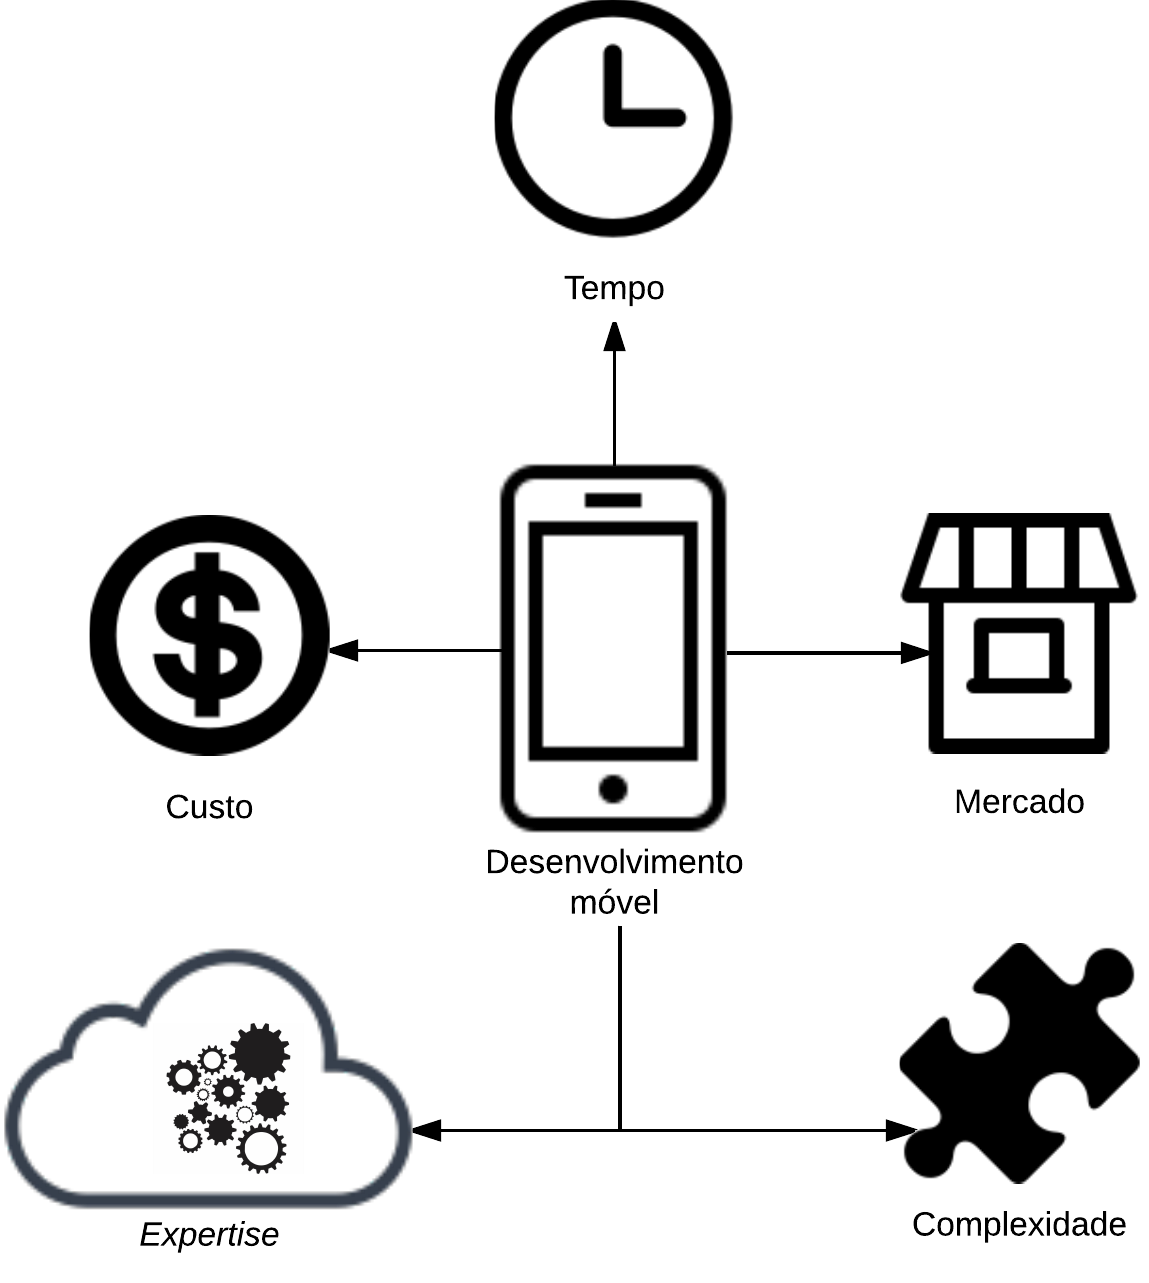
\includegraphics[width=0.55\textwidth]{analiseapp}
	\caption[Fatores a serem avaliados no desenvolvimento móvel]{ Fatores a serem avaliados no desenvolvimento móvel.}
	\label{fig:analiseapp}
\end{figure}

\begin{itemize}
    \item \textbf{Tipo e complexidade da aplicação}: cada aplicação possui requisitos diferentes e próprios que originam necessidades e dificuldades inerentes daquele aplicativo. Com isso, deve-se avaliar,
    com base nos requisitos da aplicação, qual abordagem suporta melhor o \textit{app};
    \item \textbf{\textit{Expertise} da equipe}: cada equipe possui um conjunto único de habilidades e conhecimentos. No momento da escolha de uma abordagem, esses conhecimentos
    devem ser levados em consideração, visto que é a equipe de desenvolvimento que irá conceber o produto final. Se a equipe possui mais conhecimentos em uma abordagem do que em outra, isso pode ser 
    um indicativo de qual abordagem escolher;
    \item \textbf{Nicho de mercado}: Cada plataforma móvel (iOS, Android, \textit{Windows Phone}, etc), domina uma parcela do mercado e possui um grupo de usuários com 
    características, opiniões, necessidades e gostos próprios atrelados à plataforma que usam. Com isso, no momento de criar um \textit{app} deve-se pensar para quem é esse aplicativo. Se ele for concebido 
    para suprir uma demanda de um grupo específico, talvez não haja a necessidade de criá-lo para várias plataformas;
    \item \textbf{Prazo de desenvolvimento}: Quanto mais plataformas para atender, maior é o tempo necessário para desenvolver a solução. Se o prazo do projeto for apertado para desenvolvimento de mais de uma solução 
    nativa, há de considerar o desenvolvimento multiplataforma, visto que apenas será codificada uma solução que poderá atender várias plataformas diferentes;
    \item \textbf{Capital disponível para investimento}: Desenvolver para plataformas nativas exige ambiente, infraestrutura e conhecimentos diferentes para cada plataforma. Dessa forma, quanto mais plataformas se 
    quer abarcar, mais custoso o projeto será. Uma solução multiplataforma pode ser mais viável economicamente dependendo da situação;
\end{itemize}

\section{Limitações do trabalho} \label{section:limitacoestrabalho}
Uma limitação deste trabalho é o fato da comparação entre abordagens ter sido feita considerando uma tecnologia multiplataforma baseada em componentes \textit{web}. Existem outros tipos de tecnologia multiplataforma 
que podem não se encaixar nas conclusões obtidas neste trabalho por não ficarem restritas à execução em \textit{web views}, por exemplo, o Xamarin. 

Outra limitação é o tipo de aplicativo explorado neste trabalho. Foram avaliados e desenvolvidos aplicativos de sistemas de informação móveis que acessam e mantém informações em servidores. 
Outros tipos de aplicativos como jogos e aplicações seguras, como bancos eletrônicos e mensageiros, possuem requisitos de performance e privacidade que podem impactar na avaliação das abordagens.

\section{Trabalhos Futuros} \label{section:trabalhosfuturos}
Como trabalho futuro pode-se avaliar empiricamente ferramentas para desenvolvimento multiplataforma não baseadas em tecnologias 
\textit{web}, por meio do desenvolvimento de aplicativos e da comparação destes com \textit{apps} desenvolvidos nativamente. 

Outro trabalho interessante seria realizar uma análise comparativa do desenvolvimento multiplataforma e nativo de aplicativos de 
nichos distintos aos aqui abordados, como jogos ou aplicações que possuam requisitos críticos de performance e/ou segurança.
